\chapter{纹理映射}

\textsl{纹理映射}表示物体表面细节的一幅或几幅二维图形,也称\textsl{纹理贴图}(Texture Mapping),是将纹理空间中的纹理像素映射到屏幕空间中的像素的过程,即将纹理贴图贴到三维物体表面的过程。
作用:模拟物体表面细节。

\begin{figure}[H]
    \centering
    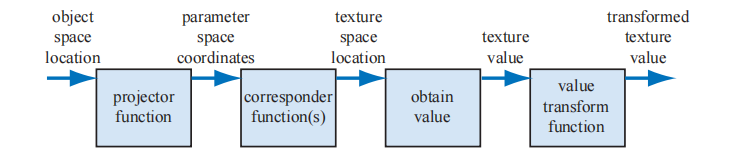
\includegraphics[scale=0.6]{figures/纹理映射的pipepine.png}
    \caption{纹理映射管线1}
\end{figure}

\begin{figure}[H]
    \centering
    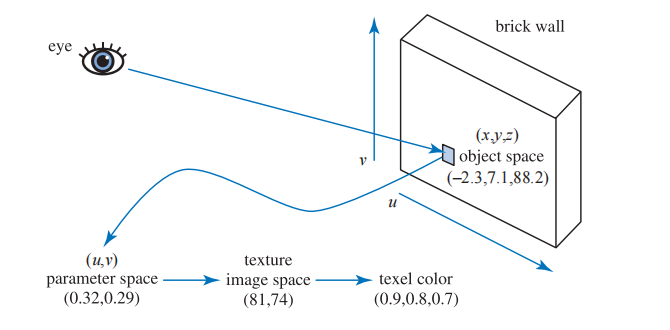
\includegraphics[scale=0.6]{figures/纹理渲染管线2.png}
    \caption{纹理映射管线2}
\end{figure}

\section{投影映射}

之所以叫投影映射,是因为主要有两种方法可以将三维的空间坐标点转化为二维的纹理坐标点:Projector 和 UV Mapping。

\begin{eqnarray}
    \phi:S\rightarrow T
\end{eqnarray}
\begin{equation}
    (x,y,z)\mapsto (u,v)
    \nonumber
\end{equation}

集合$T$称为\textsl{纹理空间},$(u,v)\in [0,1]^2$,$uv$也称为\textsl{纹理坐标},$S$是物体的坐标系。

\subsection*{Projector}

对于一些简单的几何体,通常用投影的方式

\begin{figure}[H]
    \centering
    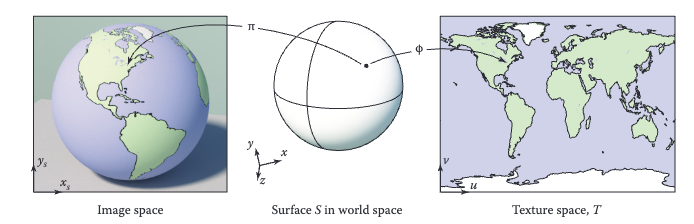
\includegraphics[scale=0.6]{figures/纹理映射.png}
    \caption{纹理映射}
\end{figure}

这种将矩形地图纹理均匀贴到球表面的投影函数称之为:Spherical 形式

此外还有 Plane, Cubic 和 Cylindrical,下图总结了四者差异(一张红绿相间的纹理贴到不同简单几何体的方式):

\subsection*{uv mapping}

Projector 只适用于简单情况,对于更复杂的几何体贴图,往往需要用到 UV Mapping:用于将 3 维模型中的每个顶点与 2 维纹理坐标一一对应。 UV map 则需要建模师精心制作。

也就是说一般情况下物体到纹理空间的纹理映射是确定好的。

\subsection*{参数化}

自动化地把复杂纹理和物体一一对应,在几何上是一个研究方向。

\section{变换函数}

\section{用重心坐标做插值}

为了兼顾功耗,很多操作都在三角形上的顶点做计算,对于三角形内部的点则通常采用插值的方法,重心坐标的作用就是脱离某个
特定坐标系去描述,方便去做插值。插值的内容可以是纹理坐标uv、颜色、法向量 等等。

为了描述一个点的位置,只需要通过下面方式描述
\begin{equation}
    (x,y)=\alpha A+\beta B+\gamma C
\end{equation}

其中如果点在三角形内,则满足$\alpha+\beta+\gamma=1$,这样就不需要通过坐标系去描述。

\subsection*{如何计算重心坐标}

首先计算重心坐标表达式中的系数\footnote{三角形重心可以把三角形分成三个等面积的三角形。}

\begin{figure}[H]
    \centering
    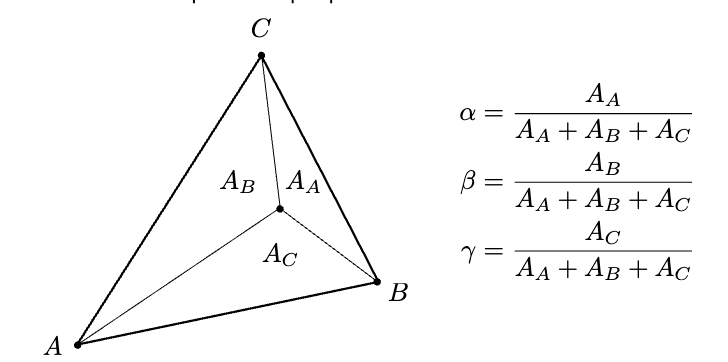
\includegraphics[scale=0.4]{figures/等面积三角形.png}
    \caption{重心坐标划分三角形区域}
\end{figure}

代入线性组合

\begin{figure}[H]
    \centering
    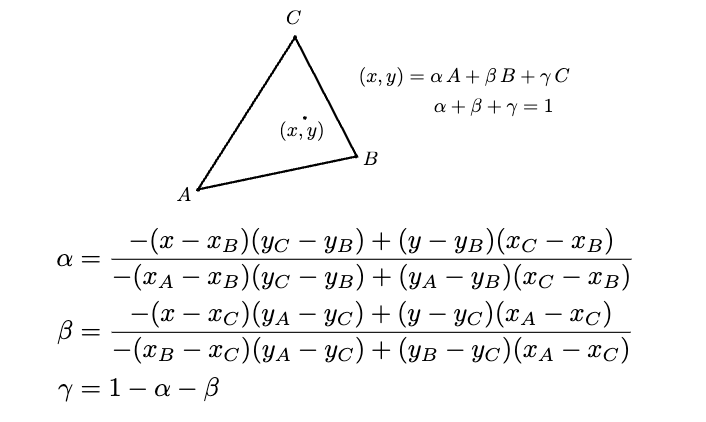
\includegraphics[scale=0.4]{figures/重心坐标2.png}
    \caption{重心坐标计算}
\end{figure}

\subsection*{利用重心坐标做插值}

\begin{figure}[H]
    \centering
    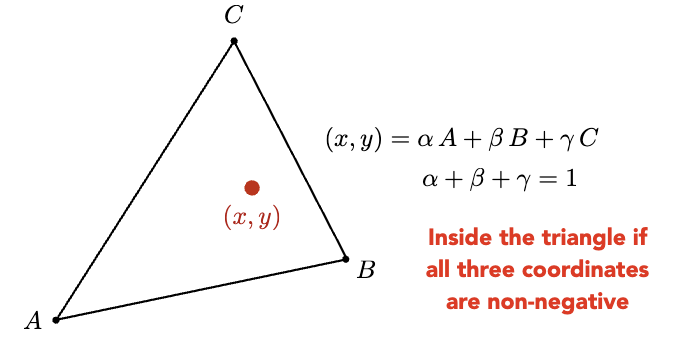
\includegraphics[scale=0.4]{figures/重心坐标1.png}
    \caption{重心坐标1}
\end{figure}

\subsection*{重心坐标不具有投影不变性}

\section{纹理放大}
纹理放大(Texture Magnification),纹理本身太小,纹理的分辨率不够,图像上的多个像素在渲染时取纹理映射上取到了同一个点,会有明显的方块状。我们将纹理上的每个像素称为texel

\subsection*{纹理小的情况}

小纹理到大分辨率屏幕之间映射会出现问题。例如256*256的纹理向4k分辨率屏幕映射的时候,原本整数的像素被压缩成小数。

\begin{figure}[H]
    \centering
    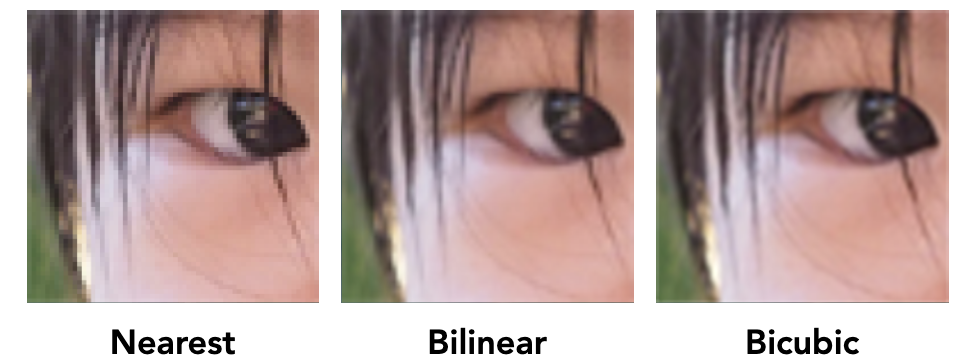
\includegraphics[scale=0.4]{figures/纹理放大.png}
    \caption{纹理放大及各种解决方式的效果}
\end{figure}

小纹理到大像素空间之间的映射本质上是高频采样低频的纹理元素,多次在一个纹理元素上进行采样造成的,因此需要对每个纹理元素之间进行插值做补正。

\subsection*{双线性插值}

\begin{figure}[H]
    \centering
    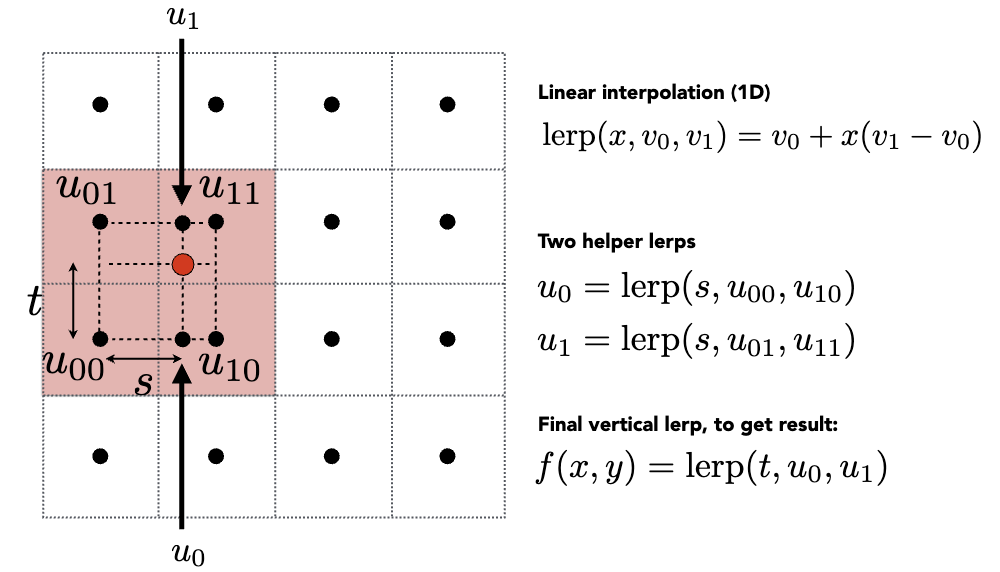
\includegraphics[scale=0.4]{figures/双线性插值补正.png}
    \caption{双线性插值补正}
\end{figure}

所谓双线性插值就是在xy两个方向上做独立地做线性插值操作。

\begin{figure}[H]
    \centering
    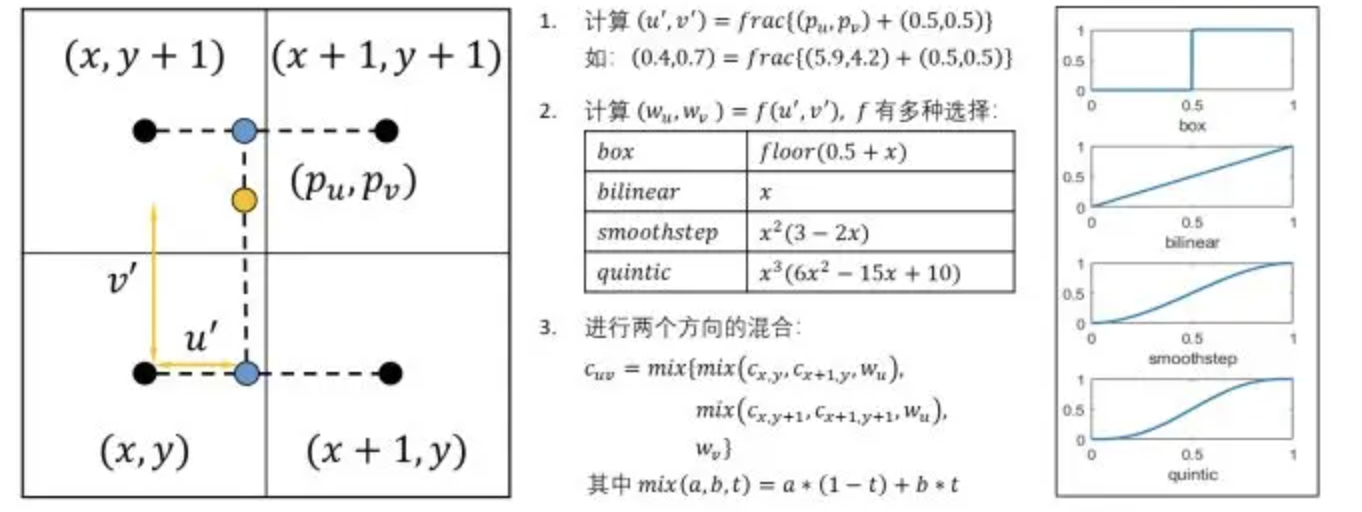
\includegraphics[scale=0.3]{figures/双线性插值流程.png}
    \caption{双线性插值流程}
\end{figure}

\subsection*{纹理大的问题}

纹理过大,导致一个pixel覆盖了多个texel,会使生成的图像产生更明显的失真。近处产生锯齿,远处摩尔纹
\footnote{在光学中,摩尔纹(Moire)是一种视觉上的干涉现象,通常在两个或多个周期性结构相互叠加时出现。当纹理较大或者具有明显的周期性结构时,往往会导致摩尔纹的产生。

摩尔纹的产生是由于两个周期性结构之间的相对位移或角度差异导致的光学干涉。当两个结构叠加在一起时,它们的周期性纹理会相互干扰,产生了一系列新的干涉纹。这些干涉纹可以表现为亮暗条纹、彩色条纹或其他形式的图案。

在纹理较大的情况下,由于纹理的周期性结构比较明显,当它们与另一个周期性结构相叠加时,干涉现象更加明显,从而产生了更为明显的摩尔纹效应。}。为什么远处会产生摩尔纹呢?
这种现象是光栅化的算法导致的。我们知道,一个三角形有顶点坐标和纹理坐标,纹理坐标范围是
[0−1][0-1][0−1]。光栅化的过程就是把三角形在屏幕上以一个个像素的形式显示出来,插值计算
三角形内部每个像素的顶点的数据,包括常见的深度值与纹理坐标。如果这个三角形距离camera近,
也就是说在屏幕上占了较多的像素,那么相邻两个像素的纹理坐标是接近的,这样通过纹理坐标获得
纹理贴图上的纹素值也是接近的,这样这俩个像素看起来比较平滑,视觉上不突兀,同时gpu读取也快
速,因为大部分纹素读取是在cache中。而如果这个三角形距离camera较远,也就是在屏幕上只占了很少
的像素,这种情况就是一个小物体应用了一个大纹理,光栅化后,相邻两个像素的纹理坐标会差别好大
,读出来的纹素也会差别很大,会很突兀,尤其是camera移动时特别明显,产生闪烁,火花现像,除
此之外,gpu读取性能也很低效,因为两个相邻的像素所对应的纹素,一个可能在cache中,另一个还没有加
载到cache中。

\begin{figure}[H]
    \centering
    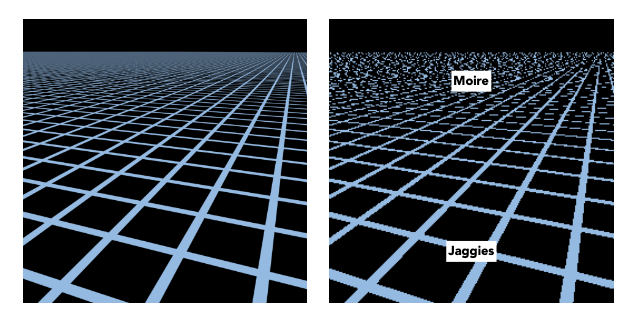
\includegraphics[scale=0.4]{figures/纹理大的情况.png}
    \caption{纹理大的情况}
\end{figure}

\subsection*{超采样}
如果一个像素不足以代表纹理的性质,那么很自然地方式是可以用超采样去解决,但是超采样是一种\textsl{点查询}解决方式,硬件开销大。

所以能否避免采样?方式就是取这个区域内的平均值。

\begin{figure}[H]
    \centering
    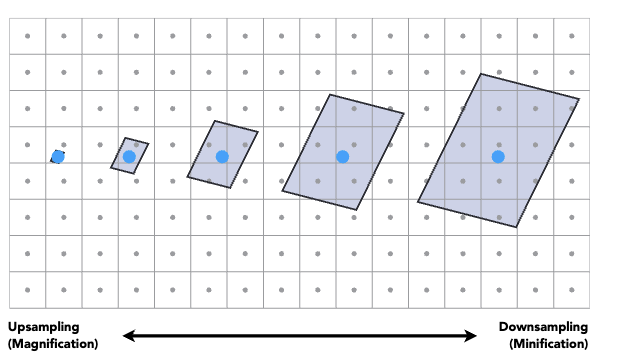
\includegraphics[scale=0.6]{figures/footprint.png}
    \caption{footprint}
\end{figure}

\subsection*{Mip-Map}

Mip-Map是一种\textsl{范围查询技术},其思想是基本思想就是,建立一系列不同尺寸的多级纹理,纹理采样时,计算对应的细节等级,再利用三线性插值计算。

\begin{figure}[H]
    \centering
    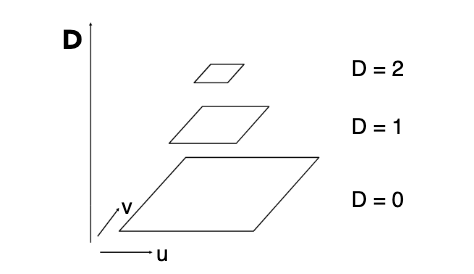
\includegraphics[scale=0.6]{figures/Mip-Map.png}
    \caption{Mip-Map纹理分层}
\end{figure}

\subsection*{各向异性过滤}



\section{帧插值技术}

\subsection*{帧插值}

\subsection*{帧采样}

\subsection*{光流法}

\section{环境光映射}

可以用纹理去描述环境光

\subsection*{Spherical Envirmental map}

环境光记录在球上会产生扭曲现象。

\subsection*{Cude mapping}

\subsection*{Bump mapping}

凹凸贴图,人为地制造法线,几何形体不变通过复杂的纹理体现物体表面的凹凸性。

如何获取这样的法线?差分获取梯度,法线垂直于梯度。

\subsection*{Displacement mapping}

改变三角形顶点的位置,代价是三角形足够细。

\section{纹理的其他应用}

\subsection*{三维空间中的噪声函数}

\subsection*{提前做着色}

环境光遮蔽

\subsection*{体渲染}
